\documentclass[spanish, fleqn]{article}
\usepackage[spanish]{babel}
\usepackage[utf8]{inputenc}
\usepackage{amsmath}
\usepackage{graphicx,float}
\usepackage{amsfonts,txfonts}
\usepackage{mathrsfs}
\usepackage[colorlinks, urlcolor=blue]{hyperref}
\usepackage{fourier}
\usepackage[top = 1.5cm, bottom = 1.5cm, left = 2cm, right = 2cm]{geometry}


\title{Presentación de Avance - Proyecto SWE \\ILI384: Taller de Modelos y Métodos Cuantitativos}
\author{Rodrigo Naranjo \and Martín Villanueva}
\date{11 de noviembre 2015}

\begin{document}
\maketitle

\thispagestyle{empty}


\section{Descripción del Problema}
El problema consiste en modelar el sistema de \textit{Shallow Water Equations} en $1D$ y $2D$, de tal modo
que se pueda determinar la evolución del sistema, dadas las ecuaciones diferenciales que modelan el problema,
las condiciones iniciales y las condiciones de borde. Las SWE corresponden a un caso particular de las ecuaciones
de Navier-Stokes, que se obtienen al hacer la suposición de que el fluido es incompresible y que no existe viscosidad, aunque esta última puede relajarse para obtener un sistema más realista. En el caso general (2D) las ecuaciones pueden 
escribirse como a continuación:
\begin{flalign}
 & \frac{\partial u}{\partial t} + u \frac{\partial u}{\partial x} + v \frac{\partial u}{\partial y} + g \frac{\partial h}{\partial x} = 0 \\
 & \frac{\partial v}{\partial t} + u \frac{\partial v}{\partial x} + v \frac{\partial v}{\partial y} + g \frac{\partial h}{\partial y} = 0 \\
 & \frac{\partial h}{\partial t} + \frac{\partial }{\partial x}(u(h-b)) + \frac{\partial }{\partial y}(v(h-b)) = 0 
\end{flalign}
donde las variables de interés (a modelar) son $h(x,y,t)$ (nivel de agua), $u(x,y,t)$ (componente de velocidad de una columna de
agua en $x$), $v(x,y,t)$ (componente de velocidad de una columna de agua en $y$). Adicionalmente deben ser conocidos $b(x,y)$ que corresponde a la \textit{batimetría} que describe la forma del fondo marino  y las condiciones de borde e iniciales del sistema.

\begin{figure}[htpb!]
\centering
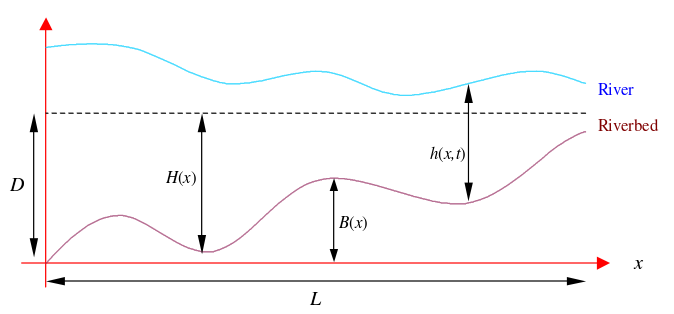
\includegraphics[scale=0.6]{schematic.png}
\caption{Esquema de SWE en una dimensión.}
\end{figure}

\section{La Implementación}
Para la resolución del problema se plantea un enfoque del tipo partículas, donde la superficie del agua se modela por medio 
de un conjunto de partículas y por la forma en que se distribuyen. Para ser más precisos, cada una de las variables de interés 
($h$, $u$ y $v$) se aproximan como una combinación lineal de funciones $RBF$. Para $h$, por ejemplo, se tiene:

$$h(x,y,t) = \sum_{i=0}^{N} \gamma_i(t)\Phi(||\mathbf{x}-\boldsymbol{\xi}_i(t)||, \epsilon_i(t))$$
 
donde la función RBF a ocupar es de preferencia una función de soporte compacto, de modo que se acote el radio de influencia 
de cada función, y se generen de este modo sistemas \textit{sparse}.

Lo que se quiere lograr sigue el enfoque \textit{Evolutive RBF}, donde se obtienen ecuaciones de evolución (ODE's) para los 
parámetros dependientes del tiempo en cada RBF ($\gamma(t)$, $\boldsymbol{\xi}_i(t)$ y $\epsilon_i(t)$). En dicho caso, para 
obtener el estado del sistema en un tiempo $t+\triangle t$, sería tan sólo computar las ecuaciones de evolución para cada RBF 
(de cada variable) y luego sumar los resultados respectivos en el espacio.

La implementación de la solución espera ser incremental, abordando la complejidad del problema paso por paso. En base a esto, se planea seguir el siguiente orden.

\begin{enumerate}
\item Inicialmente se propone resolver las \emph{Burgers' Equations} en 1D sin viscosidad, definidas por:
\begin{equation}
\frac{\partial u}{\partial t} + u\frac{\partial u}{\partial x} = 0
\label{eq:burger}
\end{equation}
que es de interés pues es no lineal y que se deriva de un modelo de convección-difusión, por lo tanto muy similar a las SWE.

\item El siguiente paso, consiste en resolver las SWE en 1D (solo se considerará el movimiento en el eje X), a modo de obtener una idea de las propiedades y comportamiento de la solución propuesta antes de avanzar a más dimensiones. Para este paso se pretende ocupar en primer lugar funciones RFB gaussianas, para luego dar con alguna implementación con funciones de soporte compacto.

\item Implementar la solución anterior al problema en 2D, considerando movimiento en el eje X e Y. 

\item Implementar condiciones de borde, iniciales y batimetría utilizadas (por otros métodos de simulación) y probarlos con esta solución para establecer comparaciones, y verificar si se están obteniendo resultados correctos.

\item Posiblemente también será necesario agregar los términos de viscosidad al sistema, para analizar sus efectos y para hacerlo más realista.

\item Buscar métodos para optimizar la ejecución de la solución encontrada: Paralelización/Implementación en GPU, Fast multipole method, aprovechar propiedades del sistema sparse, entre otras.
\end{enumerate}


\section{Dificultades}
Se presentan aquí algunas de las dificultades que se conocen, y otras que eventualmente podrían aparecer en la implementación 
del proyecto.
\begin{itemize}
	\item La batimetría $b(x,y,t)$ es, en general, una función discontinua (o que se conoce parcialmente), y por lo tanto 
	debe hallarse una manera de aproximar su derivada.
	\item En simulaciones ocupando otros métodos (SPH \textit{Smoothed Particle Hidrodynamics}) se ha notado que no tomar 
	en cuenta la viscosidad, puede llevar a problemas de estabilidad numérica en las simulaciones.
	\item Probablemente en las simulaciones sea necesario ocupar una gran cantidad de partículas para modelar la superficie
	del agua, lo cual lleva a una gran cantidad de computación para determinar los estados siguientes del sistema. Por ello,
	quizas sea necesario paralelizar la ejecución, o buscar métodos más eficientes de computación (FMM Fast Multipole 
	Method).
\end{itemize}                                                                                                                                                                                                                                                                                                                                                                                                     
\newpage  
\section{Desarrollo}
  \subsection{Burgers' Equation}
  \subsubsection{Análisis Teórico}
    Para realizar una prueba preliminar antes de modelar las SWE, se procedió a resolver la Burgers' Equation (\ref{eq:burger}), una ecuación que permite modelar de manera simplificada el comportamiento de un fluido incompresible, por medio de las leyes de la conservación. Para realizar esto se define una solución $u(x,t)$ como una combinación lineal de RBF's, del siguiente modo
    \begin{align}
      u(x,t) = \sum_{i} \Phi_i(x,t) = \sum_i \gamma_i(t)\phi_i(x-\xi_i(t),\epsilon_i)
    \end{align}
    
    Para realizar las pruebas iniciales se ocupa $\displaystyle \phi(x,\epsilon) = e^{-(\epsilon x)^2}$. Siguiendo el enfoque \textit{evolutivo} se propone $\Phi(x,t)$ (se omite subindice por simplicidad) como solución a (\ref{eq:burger}), sin embargo para abordar el problema de la no linealidad, debe hacer una modificación al problema inicial. En vista de que se propone a $\Phi(x,t)$ como una solución a la PDE, es razonable aproximar $u(x,t)$ como una expansión de Taylor en torno a $(\xi(t),t)$ obteniendo
    \begin{align}
      u(x,t) = u(\xi(t),t) + \frac{u_x(\xi(t),t)}{1!}(x-\xi(t)) + \cdots
    \end{align}
    si tomamos sólo el primer término de esta expansión (de orden cero) entonces se obtiene la equación de burger simplificada:
    \begin{align}
      \frac{\partial u}{\partial t} + u(\xi(t),t)\frac{\partial u}{\partial x} = 0
      \label{eq:burgersimple}
    \end{align}

    Luego si se reemplaza la solución propuesta $\Phi(x,t)$ en (\ref{eq:burgersimple}) se obtienen las siguientes ecuaciones de evolución para cada una de las RBF
    \begin{align*}
    & \epsilon'(t) = 0 \\
    & \gamma'(t) = 0  \\
    & \xi'(t) = u(\xi(t),t) 
    \end{align*}
    lo cual nos dice que cada una de las partículas mantendra su forma y peso, pero que sin embargo pueden cambiar su posición el tiempo, y por lo tanto la altura de la columna de agua en cada punto estará determinada sólo por la distribución de las partículas.


    \subsubsection{Análisis experimental}
    Se realizó un experimento modelando el comportamiento de la ecuación para el estado inicial:
    \begin{equation*}
      u(x) = I_{x \in [7,12]}\frac{(8-x)(x-12)}{12}
    \end{equation*} \\
    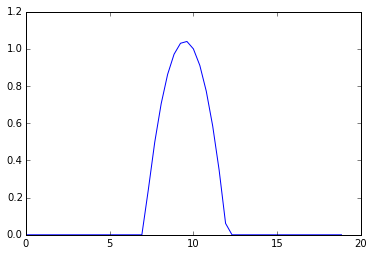
\includegraphics[scale=0.6]{initialu.png} \\

    Computando simultaneamente las ecuaciones de evolución para cada una de las RBF que componen la proximación de la solución, y luego sumando la combinación lineal en cada time step, se obtiene entonces la solución de la ecuación (\ref{eq:burgersimple}) en el tiempo. Como se vio anteriormente el único parámetro que varía en el tiempo es $\xi(t)$, que es la posición del centro de cada partícula. A continuación se muestra la evolución de cada uno de estos centros para un sistema de $20$ partículas.
    \begin{figure}
      \centering
      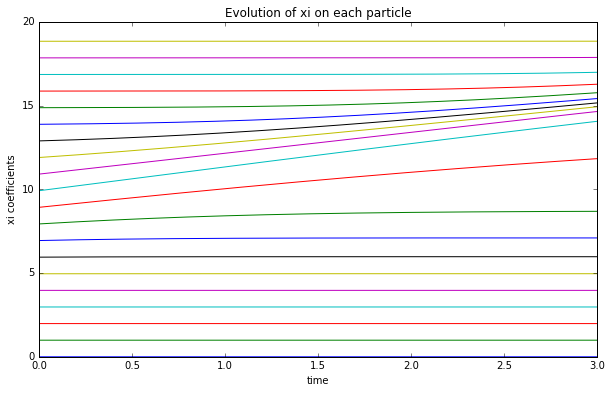
\includegraphics[scale=0.5]{xis.png}
    \end{figure}
    
    Algunos resultados obtenidos para la evolución de la ecuación en el tiempo son los que se muestran a continuación: \\
    \begin{figure}[H]
      \centering
      \begin{minipage}{.5\textwidth}
        \centering
        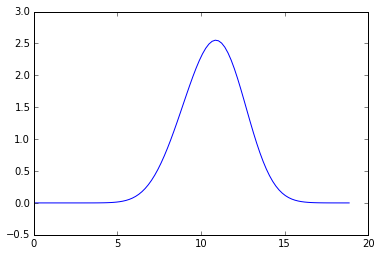
\includegraphics[scale=0.6]{t1000.png}
      \end{minipage}%
      \begin{minipage}{.5\textwidth}
        \centering
        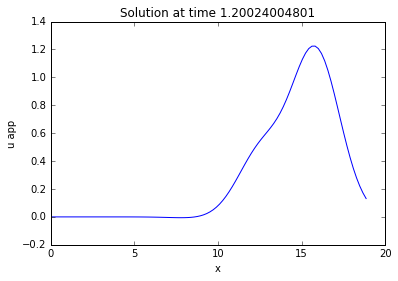
\includegraphics[scale=0.6]{t2000.png}
      \end{minipage}
    \end{figure}
    \begin{figure}[H]
      \centering
      \begin{minipage}{.5\textwidth}
        \centering
        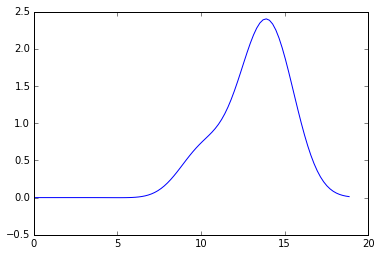
\includegraphics[scale=0.6]{t3000.png}
      \end{minipage}%
      \begin{minipage}{.5\textwidth}
        \centering
        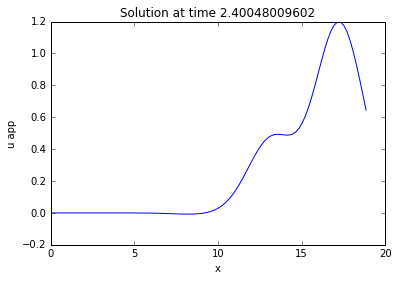
\includegraphics[scale=0.6]{t4000.png}
      \end{minipage}
    \end{figure}
    \begin{figure}[H]
      \centering
      \begin{minipage}{.5\textwidth}
        \centering
        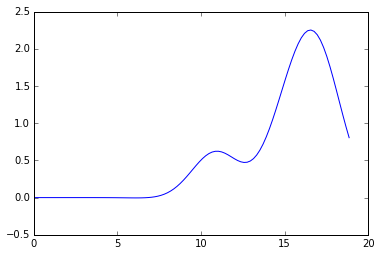
\includegraphics[scale=0.6]{t5000.png}
      \end{minipage}%
    \end{figure}
    Como se puede observar, el comportamiento modelado por la \textit{Burgers' Equation} es bastante simple, consistiendo en un
    movimiento de la perturbación inicial $u(x,0)$ acorde a su posición anterior. Algunos de los detalles que pudieron 
    observarse en la simulación son la aparición de una perturbación más pequeña que parece moverse a menor velocidad que el
    resto del sistema.
    
\vfill\hfill RN/MV/\LaTeXe
\end{document}